\documentclass[a4paper,12pt]{article}
\usepackage[utf8]{inputenc}
\usepackage[T2A]{fontenc}
\usepackage[russian,english]{babel}
\usepackage[pdftex]{graphics}
\DeclareGraphicsExtensions{.pdf,.png,.jpg}
\graphicspath{{pictures/}}
\begin{document}
\begin{center}
Санкт-Петербургский государственный политехнический университет
\\Кафедра компьютерных систем и программных технологий
\end{center}
\vspace*{10em plus .6em minus .5em}

\begin{center}
{\LARGEТелекоммуникационные технологии
\\Лабораторная работа №1
\\Визуализация сигналов во временной и частотной области}
\end{center}

\vspace*{5em plus .6em minus .5em}
\begin{flushright}
Выполнил:\\студент гр.33501/4\\Корсков Алексей\\Проверила:\\Богач Н.В.
\end{flushright}

\vspace*{15em plus .6em minus .5em}
\begin{center}
{\smallСанкт-Петербург
\\2018}
\end{center}
\pagestyle{empty}
\newpage
\pagestyle{plain}
{\bfseriesЦель}

Познакомиться со средствами генерации сигналов и визуализации их спектров.

{\bfseriesПостановка задачи}

В командном окне MATLAB и в среде Simulink промоделировать синусоидальный и прямоугольный сигналы с различными параметрами. Получить их спектры. Вывести на график.

{\bfseriesТеоретическое обоснование}

Сигналом (от лат. signum - знак) называется физический процесс или явление, несущее сообщение о каком-либо событии, состоянии объекта, либо передающее команды управления, оповещения и т.д.

{\bfseriesКлассификация сигналов}

Сигналы делятся на \textit{детерминированные} и \textit{случайные}. Детерминированные сигналы - такие сигналы, для которых мгновенные значения для любого момента времени известны и предсказуемы с вероятностью равной единице. Случайные сигналы - такие сигналы, значение которых в любой момент времени невозможно предсказать с вероятностью равной единице.

Детерминированные сигналы делятся на  \textit{периодические} и \textit{непиреодические}. К периодическим относят гармонические и полигармонические сигналы. Для периодических сигналов выполняется общее условие 
\begin{equation}
s(t) = s(t + kT),
\end{equation}
 где k = 1, 2, 3, ... - любое целое число, Т - период, являющийся конечным отрезком независимой переменной.

Сигналы могут быть \textit{аналоговыми} или \textit{дискретными}. Если сигнал можно измерять (наблюдать) в любой момент времени, то его называют аналоговым. Такой сигнал существует в любой момент времени. Дискретные сигналы могут наблюдаться и измеряться в дискретные (отдельные) ограниченные по длительности к моменту появления отрезки времени.

{\bfseriesПреобразование Фурье}

Ряд Фурье — представление функции  f с периодом $\tau$ в виде ряда
\begin{equation}
f(x) = {a_0\over 2} + \sum_{k=1}^{+\infty}A_k cos(k{2\pi\over 
\tau}x + \theta_k)
\end{equation}

Формула \textit{преобразования Фурье}:
\begin{equation}
S(\omega) = \int_{-\infty}^{\infty} s(t)e^{-j\omega t} dt.
\end{equation}
\textit{Обратное преобразование Фурье:}
\begin{equation}
s(t) = \frac{1}{2\pi} \int_{-\infty}^{\infty} S(\omega)e^{j\omega t} d\omega.
\end{equation}

Ряд Фурье является частным случаем преобразованием Фурье, но применяется когда функция периодическая. Для непериодических функций ряды Фурье неприменимы. Таким образом, преобразование Фурье ставит в соответствие сигналу, заданному во времени, его спектральную функцию. При этом говорят, то осуществляется \textit{переход из временной области в частотную}. Преобразование Фурье взаимно-однозначно, поэтому представление сигнала в частотной области (спектральная функция) содержит столько же информации, сколько и исходный сигнал, заданный во временной области.
\newpage

{\LargeХод работы}
\begin{enumerate}
{\itemПостроим синусоидальный сигнал в окне MATLAB и его спектр, с помощью следующего фрагмента кода.

\center{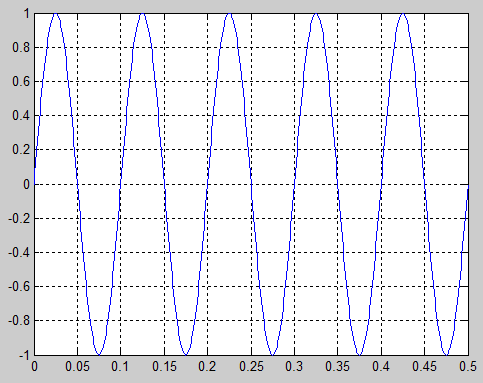
\includegraphics{./pictures/Signal.png} \\ Рис.1 Синусоидальный сигнал}
\center{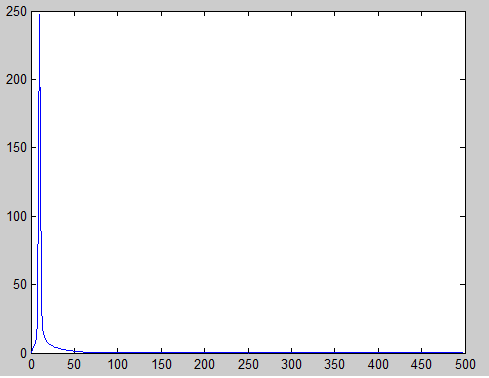
\includegraphics{./pictures/Spec.png} \\ Рис.2 Спектр синусоидального сигнала}
\\}

{\itemПостроим прямоугольный сигнал в окне MATLAB и его спектр, с помощью следующего фрагмента кода.

\center{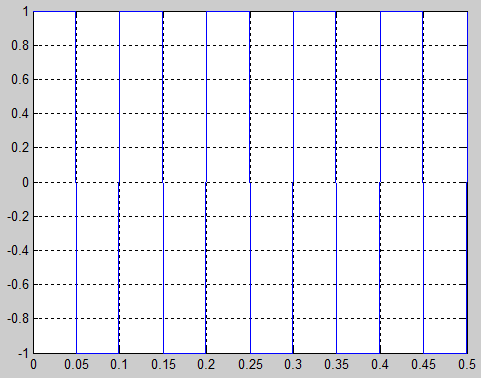
\includegraphics{./pictures/SignalN.png} \\ Рис.3 Прямоугольный сигнал}
\center{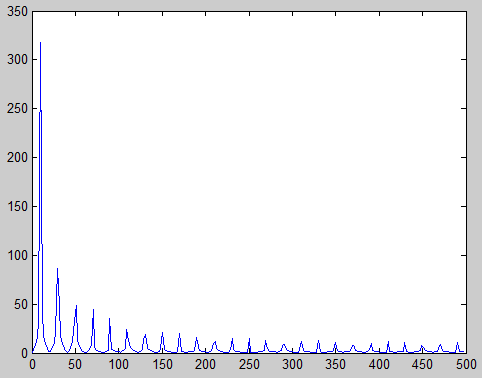
\includegraphics{./pictures/SpecN.png} \\ Рис.4 Спектр прямоугольного сигналаы}
\\}

{\itemПостроим синусоидальный сигнал и его спектр в среде Simulink. Для этого соберем следующую схему.
\center{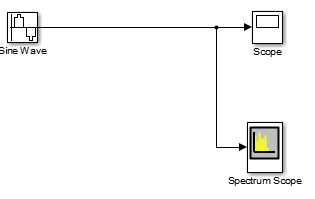
\includegraphics{./pictures/SimSin.png}}

Выходные сигналы:

\center{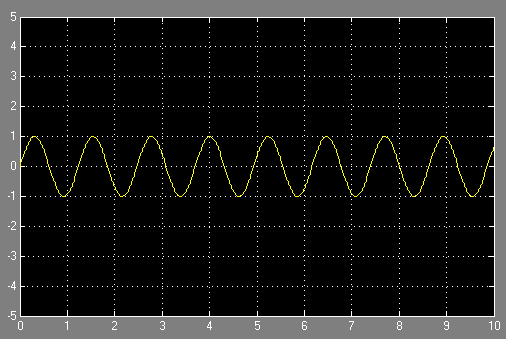
\includegraphics{./pictures/SimSignal.png} \\ Рис. 5 Визуализация синусоидального сигнала}
\center{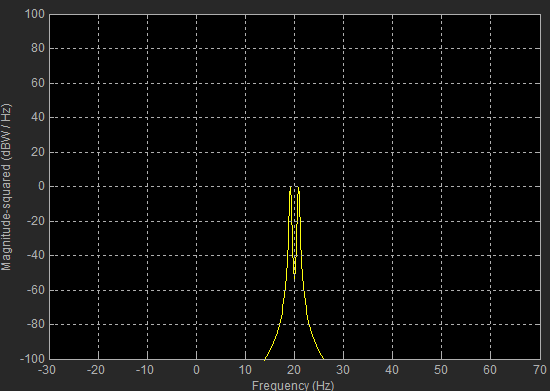
\includegraphics{./pictures/SimSpec.png} \\ Рис.6 Спектр синусоидального сигнала}
\\}

{\itemПостроим прямоугольный сигнал и его спектр в среде Simulink. Для этого соберем следующую схему.
\center{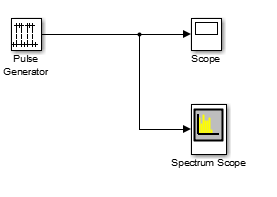
\includegraphics{./pictures/SimSinN.png}}

\begin{verbatim}
Amplitude:1
Period:2
Pulse width:1
Phase delay:0
Sample time:0.01
\end{verbatim}

Выходные сигналы:

\center{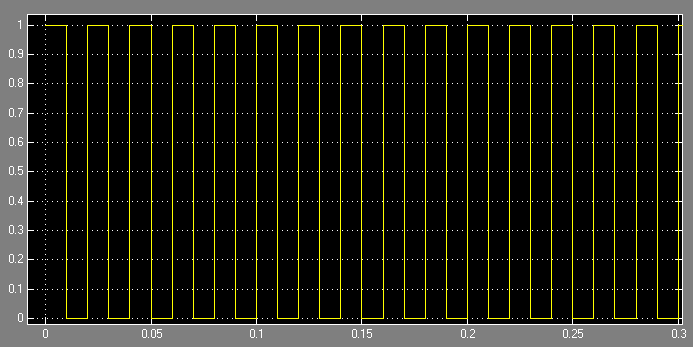
\includegraphics{./pictures/SimSignalN.png} \\ Рис. 5 Визуализация прямоугольного сигнала}
\center{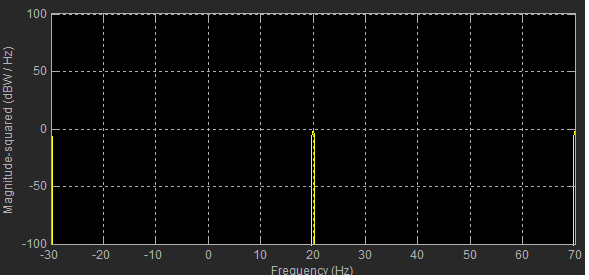
\includegraphics{./pictures/SimSpecN.png} \\ Рис.6 Спектр прямоугольного сигнала}
\\}

{\bfseries\LARGEВывод}

Была рассмотрена классификация сигналов: они делятся на \textit{периодические} и \textit{непереодические}; \textit{дискретные} и \textit{непрерывные}; \textit{бесконечные} и \textit{конечные}. Сигнал может быть представлен как во временной, так и в частотной области (спектр сигнала). Преобразование применяют потому что при анализе сигналов для одних удобнее временное отображение, а для других частотное. В данной лабораторной работе были использованы функции языка Matlab, а также средствами среды Simulink были сгенерированы и визуализированы сигналы с различными характеристиками, получены их спектры.

\end{enumerate}
\end{document}
